\chapter{Change-based Model Persistence}
\label{ch:change_based_model_persistence}
This chapter presents an approach for change-based model 
persistence, as opposed to state-based model persistence,
that can facilitate high-performance incremental model processing 
(e.g., validation, transformation,
model differencing and conflict detection) by minimising the cost 
of change identification when models evolve. 
This chapter illustrates a prototype that implements the proposed
approach on top of the Eclipse Modelling Framework.

\section{Introduction}
\label{Introduction}
To reap the benefits of Model-Based Software Engineering in the context 
of large and complex systems, the ability to process large models 
in an incremental fashion as they evolve is essential. 
Current incremental model processing techniques 
(Section \ref{sec:identifying_changes_in models}) only deliver limited 
performance benefits due to slow and imprecise model change detection 
capabilities or are limited to a single-developer environment;
not realistic for real-world software development projects.
The research introduced in this paper aims at enabling flexible 
and high-performance incremental model processing through 
change-based model persistence. That is, instead of persisting snapshots 
of the state of models, this research proposes persisting models on their change history. The proposed approach has the potential to 
deliver step-change performance benefits in incremental model processing, 
faster model differencing and conflict detection, 
as well as a wide range of other benefits and novel capabilities.

The rest of this chapter is structured as follows. 
Section \ref{sec:proposed_approach} overviews our proposed approach 
and Section \ref{sec:prototype_implementation} discusses our prototype 
implementation on top of the Eclipse Modelling Framework. 
The potential benefits and novel capabilities, as well as the challenges 
of change-based model persistence, are presented in 
Section \ref{sec:benefits_and_novel_capabilities}. Section \ref{sec:conclusions_2} concludes this chapter.

\begin{lstlisting}[style=eol,escapechar=|,caption={The complete version of Bob's change events in Listing \ref{lst:cbp_left}.},label=lst:cbp_left_full]
session "Jane-01"
create character type Class
set character.name from null to "Character" 
create attack type Operation
set attack.name from null to "attack" 
add attack to character.operations at 0
create gem type Parameter
set gem.name from null to "gem" 
add gem to attack.parameters at 0
create target type Parameter
set target.name from null to "target" 
add target to attack.parameters at 1
create weapon type Parameter
set weapon.name from null to "weapon" 
add weapon to attack.parameters at 2
create troll type Class
set troll.name from null to "Troll" 
create giant type class
set giant.name from null to "Giant"
create cast type Operation
set cast.name from null to "smash"
add cast to giant.operations at 0
create knight type Class
set knight.name from null to "Knight"
create smash type Operation
set smash.name from null to "smash"
add smash to knight.operations at 0
create mage type Class
set mage.name from null to "Mage" 
session "Bob-01"
create leftGen type Generalization
set leftGen.general from null to character
set troll.generalization to leftGen
set character.name from "Character" to "Hero"
unset troll.generalization from leftGen to null composite l1
set knight.generalization to leftGen composite l1
move target in attack.parameters from 1 to 2
unset cast.name from "cast" to null composite l2
remove cast from giant.operations at 0 composite l2
delete cast composite l2
unset giant.name from "Giant" to null composite l2
delete giant composite l2
set troll.name from "Troll" to "Ogre"
\end{lstlisting}


\section{Proposed Approach}
\label{sec:proposed_approach}

The ambition of this research is to enable high-performance incremental model management in collaborative software development environments by challenging one of the fundamental assumptions of contemporary modelling frameworks and tools: as opposed to persisting snapshots of the state of models (which is what virtually all modelling tools and frameworks currently do), this work proposes turning models inside out and persisting their change history instead.

To illustrate the proposed approach, Listing \ref{lst:xmimodel_left} shows a state-based representation of the model of Figure \ref{fig:class_diagram_left} in (simplified) XMI, and Listing \ref{lst:cbp_left} shows the proposed equivalent change-based representation of the same model. Instead of a snapshot of the state of the model, the representation of Listing \ref{lst:cbp_left} captures the complete sequence of change events (create/set/add/move/remove/delete) that were performed on the model since its creation, organised in editing sessions. There are two editing sessions in the case of this model: one in Listing \ref{lst:cbp_left} and another in Listing \ref{lst:cbp_origin}. In the actual implementation, change events in Listing \ref{lst:cbp_left} are appended to a file that is a copy of Listing \ref{lst:cbp_origin}. Listing \ref{lst:cbp_left} only shows the appended change events, while Listing \ref{lst:cbp_left_full} shows the complete change events. Replaying these changes, the change events in Listing \ref{lst:cbp_origin} first and then followed by the change events in Listing \ref{lst:cbp_left}, produces the same state as the one captured in Listing \ref{lst:xmimodel_left}. Thus, we can conclude that the proposed change-based representation carries at least as much information as the state-based representation. 

Such a representation is particularly suitable for incremental model processing. For example, if the model-to-text transformation discussed above ``remembers" that in its previous invocation it had processed up to editing session \textsf{Jane-01} (lines 1-29) of the model, it can readily identify the changes that have been made to the model since then (i.e. in session \textsf{Bob-01} -- lines 30-43) instead of having to rediscover them through (expensive) state-based model differencing.

For the sake of readability, the format of change-based persistence presented in Listing \ref{lst:cbp_left_full} is a simplified version. The real format would be something similar to the change-based file in Listing \ref{lst:class_diagram_left_cbpfile} in Appendix \ref{sec:examples_of_cbp}. For example, change event [\textsf{session "Jane-01"}] is persisted as 
\textsf{<session id="Jane-01" time="20190923181841687GMT"/>} in a real CBP file, and [\textsf{set character.name from null to "Character"}] is persisted as \textsf{<set-eattribute eclass="Class" name="name" target="character"><old-value literal=null/><value literal="Character"/></set-eattribute>}.

\section{Prototype Implementation}
\label{sec:prototype_implementation}
This work has implemented a prototype \cite{epsilonlabs2019emfcbp} of the change-based model persistence format -- the prototype is named EMF CBP -- using the notification facilities provided by the Eclipse Modelling Framework. In the implementation, the prototype uses a subclass of EMF's \textsf{EContentAdapter} (\textsf{ChangeEventAdapter}) to receive and record \textsf{Notification} events produced by the framework for every model-element level change.

\begin{figure}[th]
    \centering
    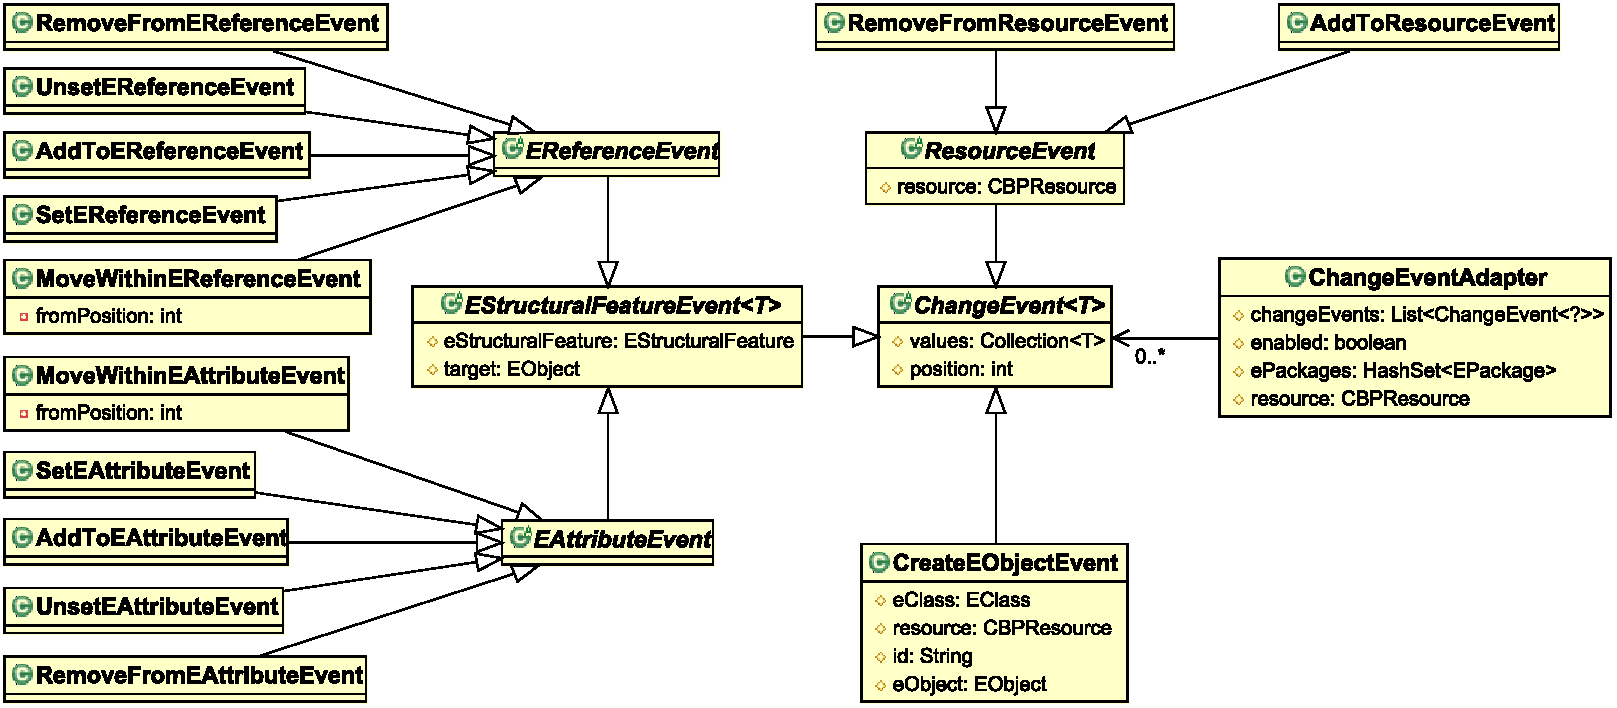
\includegraphics[width=\linewidth]{events}
    \caption{Event classes to represent changes of models.}
    \label{fig:events}
\end{figure}

Since not all change events are relevant to change-based persistence (e.g. EMF also produces change notifications when listeners/adapted are added/removed from the model), this work has defined a set of event classes to represent events of interest. The event classes are depicted in Figure \ref{fig:events} as subclasses of the \textsf{ChangeEvent} abstract class.

The \textsf{ChangeEvent} class has a multi-valued \textsf{values} attribute which can accommodate both single-valued (e.g. set/add) or multi-valued events (e.g. addAll/removeAll). \textsf{ChangeEvent} can also accommodate different types of values, such as \textsf{EObject}s for \textsf{EReferenceEvents}, and primitive values (e.g. Integer, String) for \textsf{EAttributeEvents}. The \textsf{ChangeEvent} class also has a position attribute to hold the  index of an \textsf{EObject} or a literal when they are added to a \textsf{Resource}, \textsf{EReference}, or \textsf{EAttribute} with multiple values. 

Every time an \textsf{EObject} is added to the model, a \textsf{CreateEObjectEvent} and an \textsf{AddToResourceEvent} are recorded. When an EObject is deleted, or moved to a containment \textsf{EReference} deeper in the model, a \textsf{RemoveFromResourceEvent}
 is recorded.

\vspace{-20pt}
\begin{lstlisting}[style=java,caption={Simplified Java code to handle notification events.},label=lst:javacode]
public class ChangeEventAdapter extends EContentAdapter {
...
@override
public void notifyChanged(Notification n) {
    ...
    switch (n.getEventType()) {
    ... // other events
    case Notification.UNSET: {
        if (n.getNotifier() instanceof EObject) {
            EStructuralFeature feature = (EStructuralFeature) n.getFeature();
            if (feature instanceof EAttribute) {
                event = new UnsetEAttributeEvent();
            } else if (feature instanceof EReference) {
                event = new UnsetEReferenceEvent();
            }
        } break;
    } 
    ... // other events
\end{lstlisting}	

The \textsf{ChangeEventAdapter} receives EMF change notifications in its \textsf{notifyChanged()} method and filters and transforms them into appropriate change events. As an example of how notifications are filtered and transformed, Listing \ref{lst:javacode} shows how the prototype handles \textsf{Notification.UNSET} events based on the type of the changed feature i.e. an \textsf{UnsetEAttributeEvent} is instantiated if the feature of the notifier is an \textsf{EAttribute}, or an \textsf{UnsetEReferenceEvent}  is created if the notifier is an \textsf{EReference}. The transformed instances are then stored into a list of events in \textsf{ChangeEventAdapter} (\textsf{changeEvents}) for persistence. 

To integrate seamlessly with the EMF framework and to eventually support multiple concrete change-based serialisation formats (e.g. XML-formatted representation for readability and binary for performance/size), the prototype implemented \textsf{CBPResource} abstract class, that extends EMF's built-in \textsf{ResourceImpl} class. The role of the abstract class is to encapsulate all change recording functionality while the role of its concrete subclasses is to implement serialisation and de-serialisation. For example, \textsf{CBPXMLResourceImpl} persists changes in a line-based format where every change is serialised as a single-line XML document. In this way, when a model changes, the prototype can append the new changes to the end of the model file without needing to serialise the entire model again. The prototype has also implemented a \textsf{CBPXMLResourceFactory} class that extends EMF's \textsf{ResourceFactoryImpl}, as the factory class for change-based models. Figure \ref{fig:resources} shows the relationships between these classes.

\begin{figure}[th]
    \centering
    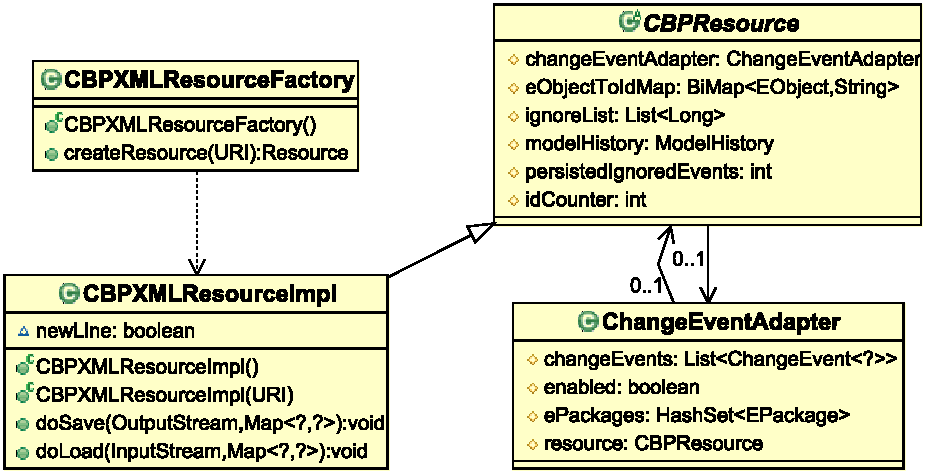
\includegraphics[width=0.75\linewidth]{resources}
    \caption{Factory, resources, and ChangeEventAdapter classes.}
    \label{fig:resources}
\end{figure}

Listing \ref{lst:javacode_resource} shows an example how to use the prototype in a Java code. Lines 1-8 demonstrate how to initialise and save a model using the prototype. First, the code creates an instance of \textsf{CBPResource}, \textsf{cbpResource}, using \textsf{CBPXMLResourceFactory} and specify its file as \textsf{helloworld.cbpxml} using \textsf{URI}. The code than executes method \textsf{startNewSession} of \textsf{cbpResource}. This methods adds a change event to indicate the start of editing session as depicted at line 1 in Listings \ref{lst:cbp_origin} and \ref{lst:class_diagram_left_cbpfile}.
The code then uses \textsf{UMLFactory} to create an element, \textsf{model}, of UML2's \textsf{Model}. The code adds element \textsf{model} into \textsf{cbpResource} and set the name to ``Hello World''. The code then saves the model in change-based format using method \textsf{save} and then unload \textsf{cbpResource}. Lines 9-12 demonstrate how to replay (load) the model that previously has been saved and then print the name of the first element in \textsf{cbpResource} which is expected to print ``Hello World'' text.

\vspace{-20pt}
\begin{lstlisting}[style=java,caption={An example how to use \textsf{CBPResource} in Java code.},label=lst:javacode_resource]
/* initialise, save, and unload */
CBPResource cbpResource = (CBPResource) (new CBPXMLResourceFactory()).createResource(URI.createFileURI("helloworld.cbpxml"));
cbpResource.startNewSession("Initial");
Model model = UMLFactory.eINSTANCE.createModel();
cbpResource.getContents().add(model);
model.setName("Hello World");
cbpResource.save(null);
cbpResource.unload();

/* load and print */
cbpResource.load(null);
model = (Model) cbpResource.getContents().get(0);
System.out.println(model.getName()); // expected output: "Hello World"
\end{lstlisting}

\section{Benefits and Novel Capabilities}
\label{sec:benefits_and_novel_capabilities}
Beyond facilitating incremental processing, the proposed representation 
also has the potential to deliver a wide range of benefits and 
novel capabilities, compared to the currently prevalent 
state-based representations, some of which are discussed below.

\begin{itemize}
    \item With appropriate tool support, modellers will be able to ``replay" (part of) the change history of a model (e.g. to understand design decisions made by other developers, for training purposes). In state-based approaches, this can be partly achieved if models are stored in a version-control repository (e.g. Git). However, the granularity would only be at the commit level.
    \item By analysing models serialised in the proposed representation, modelling language and tool vendors will be able to develop deeper insights into how modellers actually use these languages/tools in practice and utilise this information to guide the evolution of the language/tool.
    \item By attaching additional information to each session (e.g. the id of the developer, references to external documents/URLs), sequences of changes can be traced back to the developer that made them, or to requirements/bug reports that triggered them.
    \item Persisting changes to large models after an editing session will be significantly faster compared to serialising the entire state of the model, as only changes made during the session will need to be appended to the model file.
    \item The performance and precision of model comparison and merging can be substantially improved, particularly for large models with shared editing histories.
\end{itemize}

\section{Challenges}
\label{sec:challenges}
The proposed approach also comes with a number of challenges that this research will need to overcome, such as loading overhead and fast-growing model files. However, due to limitation of time, this work only addresses the loading overhead while the fast-growing model files is set as another topic for future work.  

While, as discussed above, persisting changes to large models is expected to be much faster and resource-efficient compared to state-based approaches, loading models into memory by naively replaying the entire change history is expected to have a significant overhead. To address this challenge, this work has developed two solutions that reduces the cost of change-based model loading, firstly, by recording and ignoring events -- events that are later overridden or cancelled out by other events -- and, secondly, by proposing a hybrid model persistence format which models are loaded from stated-based persistence but changes are persisted into both change-based and state-based representation. 

For the fast-growing model files challenge, persisting models in a change-based format means that model files will keep growing in size during their evolution significantly faster than their state-based counterparts. To address this challenge, one can proposes sound change-compression operations (e.g. remove older/unused information) that can be used to reduce the size of a model in a controlled way or develops a compact textual format that will minimise the amount of space required to record a change (a textual line-separated format is desirable to maintain compatibility with file-based version control systems).  

\section{Conclusions}
\label{sec:conclusions_2}
Through persisting models' change history, this research aims at enabling high-performance incremental model processing in collaborative development settings. The proposed approach also has the potential to enable model analytics, more fine-grained tracing, and to improve the precision and performance of model comparison and merging. A prototype implementation of a change-based persistence format has been presented and the main envisioned challenges have been listed. 